\scanpage{26}
\diagram{\begin{tikzcd}[column sep=large]
\begin{gathered}\text{Carte cellulaire (pas orientée) }\unsure{\text{conn}}\\
\text{dont tous les sommets sont}\\
\text{d'ordre }3\ \inserted{\text{ou }1}
\end{gathered}
\arrow[r,leftrightarrow] & \text{Cartes }\uline{\text{cellulaires}}
\end{tikzcd}}
\margin{\(\unsure{\mathrm{or}^{t}}\)}
triangulée \(\simeq\)
\margin{\(\deleted{\unsure{\mathbf Z}}\unsure{n-}\)}
revêtements de \(\mathbb P^1_{\unsure{\mathbb Q|\mathbb C}}\) ramifiés \unsure{seulement} en \(0,1,\infty\),
\figure{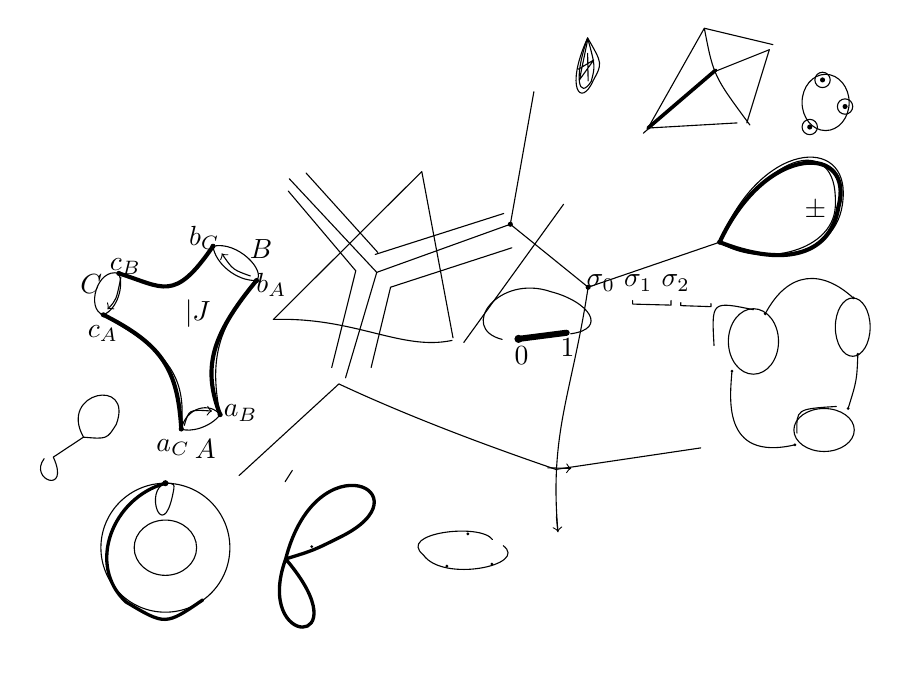
\begin{tikzpicture}[x=.0065cm,y=-.0065cm,line cap=round,line join=round]
\begin{scope}[shift={(1112,150)}]
\draw (0,-55) .. controls (-45,43) and (-13,83) .. (11,28) .. controls (29,-5) .. (0,-55);
\draw (0,-55) .. controls (-28,24) and (-17,67) .. (7,30) .. controls (15,0) .. (0,-55);
\draw (0,-51)--(-16,27)--(12,-12)--(-18,6) (0,-25)--(1,29);
\end{scope}
\begin{scope}[shift={(1340,170)}]
\draw (-110,101)--(0,-94)--(134,-62) (127,-52)--(83,91) (0,-94)..controls (18,-1)..(89,95) (-110,101)--(64,91);
\draw[line width=1.3pt] (-110,101)--(22,-12);
\draw (-119,111)--(17,-8)--(127,-52);
\end{scope}
\begin{scope}[shift={(1577,221)}]
\draw (0,0) ellipse (46 and 55);
\foreach \x/\y in {-6/-44,38/8,-31/48}{\draw (\x,\y) circle (15);\fill (\x,\y) circle (5);}
\end{scope}
\begin{scope}[shift={(300,680)}]
\draw[line width=1.5pt] (-104,-125) .. controls (-17,-98) and (4,-67) .. (80,-178);
\draw[line width=1.5pt] (165,-111) .. controls (74,-1) and (60,62) .. (94,151);
\draw[line width=1.5pt] (-134,-44) .. controls (-17,15) and (11,64) .. (18,179);
\draw (-139,-45) .. controls (-9,26) and (29,74) .. (18,179);
\draw (165,-111) .. controls (99,-28) and (69,29) .. (94,151);
\draw (-104,-125) .. controls (-147,-137) and (-169,-54) .. (-134,-44) .. controls (-106,-56) and (-94,-101) .. (-104,-125);
\draw (80,-178) .. controls (128,-189) and (184,-130) .. (165,-111) .. controls (124,-110) and (84,-146) .. (80,-178);
\draw (18,179) .. controls (28,136) and (74,126) .. (94,151) .. controls (74,177) and (34,186) .. (18,179);
\draw[->] (153,-120) .. controls (119,-132) .. (97,-164);
\draw[->] (-100,-117) .. controls (-109,-73) .. (-126,-55);
\draw[->] (24,172) .. controls (33,141) .. (78,144);
\foreach \x/\y in {-104/-125,-134/-44,80/-178,165/-111,18/179,94/151}{\fill (\x,\y) circle (5);}
\node at (-158,-105) {\(C\)};
\node at (174,-172) {\(B\)};
\node at (65,218) {\(A\)};
\node at (-91,-138) {\(c_B\)};
\node at (-135,-8) {\(c_A\)};
\node at (63,-195) {\(b_C\)};
\node at (194,-103) {\(b_A\)};
\node at (134,148) {\(a_B\)};
\node at (2,216) {\(a_C\)};
\node at (50,-47) {\(\unsure{\circlearrowleft|J}\)};
\end{scope}
\draw (529,370)--(700,553)--(639,759) (562,359)--(702,514) (527,394)--(659,550)--(612,739);
\draw (689,739)--(727,582)--(964,505) (700,553)--(961,459) (697,518)--(948,438);
\draw (498,645)--(788,356)--(849,681);
\draw (498,645) .. controls (658,640) and (748,707) .. (847,686);
\draw (870,690)--(1065,420);
\draw (1007,200)--(961,459)--(1113,582)--(1370,494);
\draw (1113,582) .. controls (1081,793) and (1037,863) .. (1054,1060);
\draw (431,950)--(626,771) .. controls (780,843) and (945,902) .. (1050,938)--(1333,896);
\draw[->] (1034,935)--(1080,936);
\draw[->] (1051,1030)--(1054,1060);
\foreach \x/\y in {961/459,1113/582,1370/494}{\fill (\x,\y) circle (5);}
\begin{scope}[shift={(1370,494)}]
\draw[line width=1.5pt] (0,0) .. controls (91,-197) and (266,-191) .. (232,-69) .. controls (216,33) and (115,46) .. (0,0);
\draw (0,0) .. controls (103,-191) and (229,-203) .. (226,-79) .. controls (231,19) and (78,52) .. (0,0);
\draw (0,0) .. controls (79,-198) and (253,-210) .. (241,-84) .. controls (232,40) and (78,42) .. (0,0);
\node at (187,-61) {\(\pm\)};
\end{scope}
\node at (1211,574) {\(\sigma_0\ \sigma_1\ \sigma_2\)};
\draw (1200,608)--(1200,615)--(1275,617)--(1275,608) (1294,612)--(1294,618)--(1353,620)--(1353,614);
\draw (945,684) .. controls (858,662) and (938,555) .. (1041,591) .. controls (1114,610) and (1153,663) .. (1079,673);
\draw[line width=2.2pt] (977,683)--(1071,671);
\fill (977,683) circle (8);
\node at (983,715) {\(0\)};
\node at (1073,700) {\(1\)};
\begin{scope}[shift={(1510,739)}]
\draw (-51,-105) .. controls (-6,-190) and (60,-192) .. (121,-136);
\draw (130,-26) .. controls (128,25) .. (111,80);
\draw (7,151) .. controls (-139,185) and (-119,53) .. (-116,7);
\draw (-74,-51) ellipse (49 and 64);
\draw (120,-79) ellipse (34 and 57);
\draw (64,122) ellipse (59 and 42);
\draw (-74,-113) .. controls (-156,-130) .. (-151,-43);
\draw (11,128) .. controls (10,81) .. (88,76);
\foreach \x/\y in {-51/-105,-116/7,121/-136,130/-26,111/80,7/151}{\fill (\x,\y) circle (3);}
\end{scope}
\draw (127,875) .. controls (77,786) and (226,757) .. (191,850) .. controls (173,879) .. (127,875)--(68,914) .. controls (102,988) and (19,959) .. (50,917);
\begin{scope}[shift={(287,1091)}]
\draw (0,0) ellipse (126 and 126);
\draw (0,0) ellipse (61 and 54);
\draw[line width=1.2pt] (0,-126) .. controls (-105,-97) and (-154,35) .. (-77,106) .. controls (0,152) .. (73,102);
\draw (0,-126) .. controls (-42,-113) and (-6,-9) .. (14,-102) .. controls (19,-126) .. (0,-126);
\fill (0,-126) circle (6);
\end{scope}
\begin{scope}[shift={(522,1113)}]
\draw[line width=1.2pt] (0,0) .. controls (61,-237) and (282,-129) .. (107,-43) .. controls (55,-17) .. (0,0) .. controls (-64,177) and (152,178) .. (0,0);
\fill (51,-24) circle (3);
\end{scope}
\draw (791,1105) .. controls (738,1062) and (903,1042) .. (926,1075);
\draw (947,1087) .. controls (998,1125) and (829,1160) .. (791,1105);
\foreach \x/\y in {878/1064,837/1127,925/1123}{\fill (\x,\y) circle (3);}
\draw (521,962)--(535,940);
\end{tikzpicture}}% crop-candidate: scan 26
\deleted{\unsure{cartes sphériques} \unsure{d}}
\[
\sigma_0^2=\sigma_1^2=\sigma_2^2=(\sigma_0\sigma_2)^2=(\sigma_0\sigma_1)^3=1
\]
\(\mathbb R\)-cartes \unsure{rigidifiées}
\margin{\(\sigma_0,\sigma_1,\sigma_2\)\quad \unsure{ses} pts fixes}
\margin{25}
